\documentclass[11pt]{article}
\usepackage[margin=1in]{geometry}
\usepackage[T1]{fontenc}
\usepackage{lmodern}
\usepackage{microtype}
\usepackage{amsmath,amssymb,mathtools}
\usepackage{booktabs,tabularx,array}
\usepackage{graphicx}
\usepackage{tikz}
\usetikzlibrary{arrows.meta,positioning,shapes.geometric,calc,fit}
\usepackage{caption}
\usepackage[hidelinks]{hyperref}
\usepackage{xcolor}
\usepackage{enumitem}
\setlist{nosep}
\setlength{\emergencystretch}{2em}
\captionsetup{font=small,labelfont=bf}

\title{RAKL: An Evidence-Governed Recursive Atlas Method for Scientific Research with Large Language Models}
\author{Sze Chun Yiu}
\date{10 August 2026}

\newcommand{\RAKL}{\textsc{RAKL}}
\newcommand{\CannotCheck}{\texttt{CANNOT\_CHECK}}
\newcommand{\CannotCompile}{\texttt{CANNOT\_COMPILE}}
\newcommand{\SoftwareTests}{614}
\newcommand{\ImplementationSHA}{\texttt{0b6f83581bdfd2900e38a9b6af4672ac03b75f39}}

\begin{document}
\maketitle

\begin{abstract}
Large language models can search literature, generate hypotheses, execute analyses and draft research reports, while recent systems increasingly automate end-to-end scientific workflows. Fluency and workflow completion, however, do not determine which generated statements deserve scientific authority, whether apparently conflicting studies share a context, whether predictive agreement identifies a mechanism, or whether a self-modifying research agent improved beyond the benchmark it optimized. We introduce \RAKL{} (Recursive Atomic Knowledge Lattices), a candidate evidence-governed methodology for LLM-mediated scientific inquiry. \RAKL{} represents research as controlled updates to an external contextual Knowledge Atlas. Local scientific charts carry evidence, context and multi-axis authority certificates; typed transitions separate representation, prediction, mechanism, identification and decision claims; incompatible local views can remain a plural atlas or identified set rather than being forcibly merged. Residuals open recursive atomic research fibers, negative evidence is immutable history, and stopping depends on semantic novelty and evidence-lineage independence. A bounded context compiler exposes only an epistemically mandatory working set to the LLM, decoupling archive growth from prompt growth. The method is also applied to itself: challenge learning, external-method assimilation and constructive invention may propose changes, but strong self-evolution evidence requires frozen development tests, fresh assurance and a protected evaluator. The current reference profile assigns explicit contracts to 24 high-impact research-method surfaces and includes executable measurement/uncertainty, context-efficiency, model-criticism and assumption-sensitivity support. On exact implementation candidate \ImplementationSHA{}, the software suite passed \SoftwareTests{} tests. Same-context Self-\RAKL{} has exposed and repaired several framework defects; we treat this as first-sign self-correction rather than independent self-evolution. A preregistered quantitative-finance trial will use the framework to construct a descriptive and predictive model of 5- and 15-minute cryptocurrency spot movement, with Polymarket strictly downstream of spot-model validation.
\end{abstract}

\section{Introduction}
Scientific-agent systems have moved rapidly beyond question answering. Co-Scientist combines generation, reflection, ranking and hypothesis evolution and includes experimental biomedical validation \cite{gottweis2026}; Robin integrates literature and data-analysis agents across a discovery workflow \cite{ghareeb2026}; AI Scientist-v2 automates experiment design, execution, analysis and paper generation using agentic tree search \cite{yamada2025}; Kosmos uses a structured world model for long-horizon discovery \cite{mitchener2025}; SciAgents couples multi-agent reasoning with ontological knowledge graphs \cite{ghafarollahi2024}; and PaperQA2 demonstrates strong agentic literature synthesis \cite{skarlinski2024}. These systems make it untenable to position a new method as novel merely because it searches papers, generates hypotheses, uses multiple agents, retains research state or iteratively revises ideas.

A recent evaluation spanning more than 25,000 scientific-agent runs reported frequent evidence neglect and relatively infrequent refutation-driven revision, illustrating that workflow success and epistemically self-correcting reasoning are different targets \cite{riosgarcia2026}. The remaining problem is therefore narrower: \emph{what is a new observation allowed to change in the scientific state?} Two papers can use the same terminology while describing different populations, scales or measurement operators. Two models can be observationally equivalent yet mechanistically distinct. A model can be decision-useful while its microscopic mechanism remains unidentified. Several papers or agents can appear independent while sharing evidence lineage. A null result can disappear after enough iterations. A loop can stop because its resource budget is exhausted rather than because the scientific search has become semantically flat. A self-modifying agent can overfit the very evaluator used to declare its improvement.

\RAKL{} treats these as failures of \textbf{epistemic state transition}. The language model is a replaceable proposer. Canonical scientific state lives outside the model and changes only through evidence- and governance-bearing transitions. Scientific knowledge is represented as an atlas of contextual local views rather than one accumulating natural-language answer. The same evidence discipline is applied recursively to candidate changes in the research method itself.

This preprint makes five candidate contributions. First, it specifies a projection-first scientific state in which source claims become context-scoped local charts before they compete. Second, it provides a typed transition and obstruction discipline that separates local compatibility, path coherence, global existence and global identifiability. Third, it represents scientific authority as a multi-axis partial order rather than a scalar confidence. Fourth, it couples recursive fibers, negative history, semantic/evidence-lineage stopping, bounded epistemic context, metacognitive learning and governed method evolution in one control architecture. Fifth, it makes these claims falsifiable through machine-checkable method contracts, hostile known-answer worlds, a frozen self-bootstrap protocol and a preregistered real scientific application.

We do not claim novelty for multi-agent science, knowledge graphs, provenance, sheaf-like local-to-global reasoning, hierarchical memory, prompt compression, active experiment design, causal discovery, skill libraries or program evolution in isolation. The candidate contribution is the integrated evidence-governed transition discipline connecting them.

\begin{figure}[t]
\centering
\resizebox{\textwidth}{!}{%
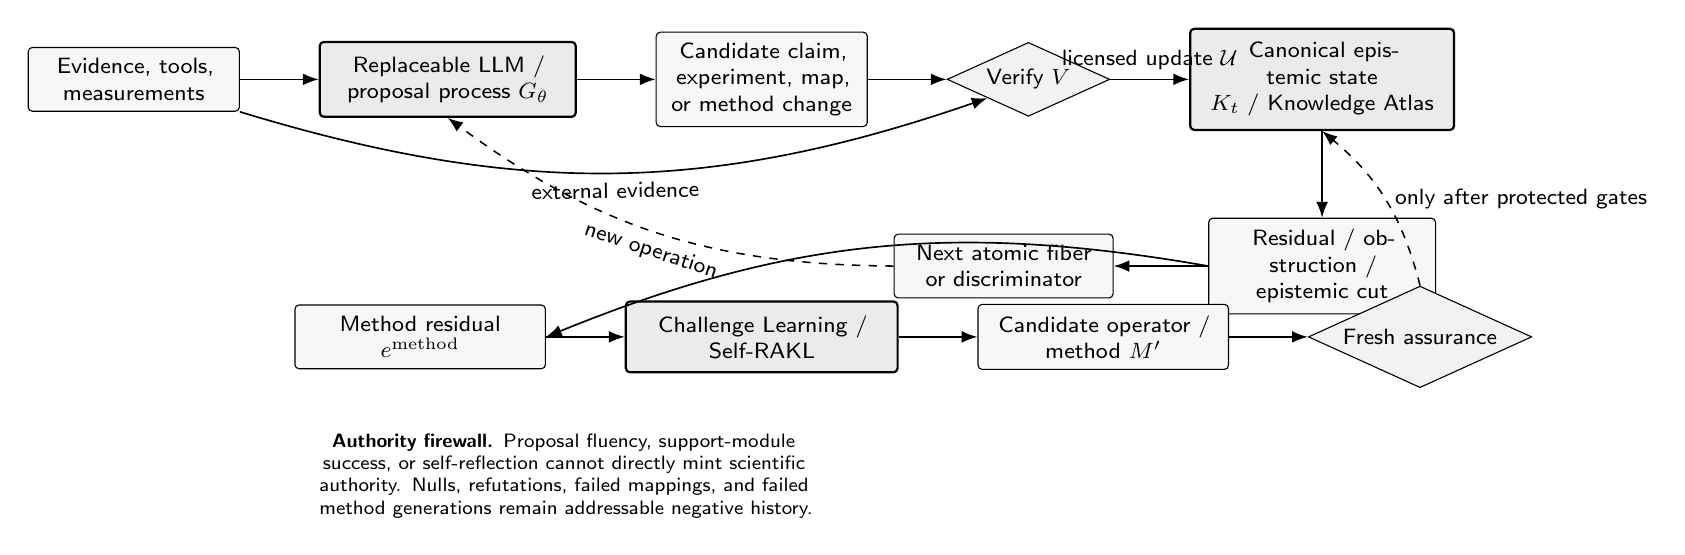
\begin{tikzpicture}[
  node distance=8mm and 10mm, >=Latex,
  every node/.style={font=\sffamily\footnotesize,align=center},
  box/.style={draw,rounded corners=1.5pt,minimum height=8mm,inner sep=4pt,fill=black!3},
  strong/.style={draw,rounded corners=1.5pt,minimum height=9mm,inner sep=5pt,line width=0.8pt,fill=black!8},
  gate/.style={draw,diamond,aspect=2.2,inner sep=2pt,fill=black!5},
  arrow/.style={->,line width=0.6pt}, dashedarrow/.style={->,dashed,line width=0.55pt}]
\node[box,text width=24mm] (evidence) {Evidence, tools,\\measurements};
\node[strong,text width=29mm,right=of evidence] (proposer) {Replaceable LLM /\\proposal process $G_\theta$};
\node[box,text width=24mm,right=of proposer] (proposal) {Candidate claim,\\experiment, map,\\or method change};
\node[gate,right=10mm of proposal] (verify) {Verify $V$};
\node[strong,text width=30mm,right=10mm of verify] (state) {Canonical epistemic state\\$K_t$ / Knowledge Atlas};
\draw[arrow] (evidence) -- (proposer); \draw[arrow] (proposer) -- (proposal); \draw[arrow] (proposal) -- (verify);
\draw[arrow] (evidence.south east) to[bend right=18] node[below,sloped]{external evidence} (verify.south west);
\draw[arrow] (verify) -- node[above]{licensed update $\mathcal U$} (state);
\node[box,text width=26mm,below=11mm of state] (residual) {Residual / obstruction /\\epistemic cut};
\node[box,text width=25mm,left=12mm of residual] (action) {Next atomic fiber\\or discriminator};
\draw[arrow] (state) -- (residual); \draw[arrow] (residual) -- (action);
\draw[dashedarrow] (action.west) to[bend left=18] node[below,sloped]{new operation} (proposer.south);
\node[strong,text width=31mm,below=22mm of proposal] (meta) {Challenge Learning /\\Self-RAKL};
\node[box,text width=29mm,left=of meta] (methodres) {Method residual\\$e^{\mathrm{method}}$};
\node[box,text width=29mm,right=of meta] (candidate) {Candidate operator /\\method $M'$};
\node[gate,right=10mm of candidate] (assure) {Fresh assurance};
\draw[arrow] (residual.west) to[bend right=16] (methodres.east); \draw[arrow] (methodres) -- (meta); \draw[arrow] (meta) -- (candidate); \draw[arrow] (candidate) -- (assure);
\draw[dashedarrow] (assure.north) to[bend right=18] node[right]{only after protected gates} (state.south);
\node[font=\sffamily\scriptsize,anchor=north west,text width=66mm] at ([yshift=-7mm]methodres.south west) {\textbf{Authority firewall.} Proposal fluency, support-module success, or self-reflection cannot directly mint scientific authority. Nulls, refutations, failed mappings, and failed method generations remain addressable negative history.};
\end{tikzpicture}}
\caption{\textbf{RAKL separates proposal generation from scientific authority.} Evidence and tools inform a replaceable proposer, but candidate claims and method changes pass through explicit verification before canonical state can change. Residuals drive scientific fibers; method residuals can trigger Challenge Learning and Self-RAKL, but fresh assurance is outside the challenger's write authority.}
\label{fig:architecture}
\end{figure}

\section{Related work and novelty boundary}
Self-improving agents and reusable skills are established directions. Darwin G\"odel Machine iteratively modifies agent code and empirically selects descendants \cite{zhang2025}. EvoSkill uses failure analysis, held-out validation and a Pareto skill archive \cite{alzubi2026}. SkillFoundry builds and evolves scientific skill libraries from heterogeneous resources \cite{shen2026}. EvoAgentBench explicitly evaluates self-evolution through ability transfer \cite{gao2026}. Consequently, \RAKL{} does not claim novelty for recursive modification, failure-driven skill creation or held-out skill transfer.

Local-to-global consistency has a long mathematical history; recent sheaf work gives conditions under which compatible engineering views glue uniquely \cite{gibson2026}. Provenance-centered knowledge models preserve attributed local worlds rather than forcing every statement into one global fact set \cite{vitali2026}. Agent-workflow provenance and verifiable agent-native publishing are also active research topics \cite{souza2025,dogah2026}. \RAKL{} uses these as prior mechanisms and claims only the narrower integration with scoped authority, residual routing and governed state transitions.

Hierarchical memory and context optimization are also prior art. MemGPT frames long-horizon context as a virtual-memory problem \cite{packer2023}; RAPTOR organizes multi-resolution retrieval hierarchically \cite{sarthi2024}; LLMLingua compresses prompts \cite{jiang2023}; and RECOMP selectively compresses retrieved evidence \cite{xu2023}. \RAKL{} therefore does not claim generic compression or hierarchical memory. Its narrower requirement is that a context policy preserve registered mandatory epistemic material or fail closed.

\section{Formal method}
\subsection{Task, researcher state and epistemic state}
A scoped inquiry is
\begin{equation}\mathcal P=(O,\mathcal Q,\Gamma_0,\mathcal E_0,\mathcal B,\Lambda),\end{equation}
where $O$ is the target object, $\mathcal Q$ the registered scientific questions or quantities of interest, $\Gamma_0$ the context/observation boundary, $\mathcal E_0$ the evidence available at the declared cutoff, $\mathcal B$ the resource budget and $\Lambda$ the blocking epistemic invariants.

The functional researcher state is
\begin{equation}\mathfrak R_t=(K_t,\mathcal Z_t,\Omega_t,\Pi_t,\mathcal G_t,\mathcal M_t,\mathcal X_t,\mathcal R_t),\end{equation}
separating canonical scientific state, explanatory models, method skills, executive policy, research agenda, metacognition, experience/transfer history and resources. The epistemic state is
\begin{equation}K_t=(\mathcal A_t,\mathcal T_t,\mathcal V_t,\mathcal E_t,\mathcal U_t,\mathcal O_t,\mathcal F_t,\mathcal H_t^{-},\mathcal S_t,\mathcal G_t^K),\end{equation}
with Knowledge Atlas charts, typed transitions, survivors, evidence/provenance, uncertainty and identified sets, obstructions/residuals, recursive fibers, immutable negative history, saturation state and protected governance identity.

\subsection{Contextual charts, transitions and gluing}
A local scientific chart is
\begin{equation}C_i=(U_i,\phi_i,\gamma_i,e_i,\alpha_i),\end{equation}
where $\gamma_i$ can include population, scale, regime, units, observation model, assumptions, intervention, time/cutoff and QoI. Source observations are contextual projections $y_i=\pi_i(O\mid\gamma_i)$ rather than globally competing whole-object answers.

For overlapping charts,
\begin{equation}T_{ij}^{\tau,\sigma}:\phi_i(U_i\cap U_j)\rightarrow\phi_j(U_i\cap U_j)\end{equation}
is a typed, scoped transition carrying evidence, assumptions and uncertainty semantics. Composition is licensed only when interfaces, relation types, scopes, invariants, lineage and error-composition rules are compatible. Graph connectivity alone does not create endpoint scientific authority.

At comparison layer $\ell$, a contradiction requires overlap, alignment and incompatibility:
\begin{equation}\operatorname{Contradict}_{\ell}(C_i,C_j)=\operatorname{Overlap}(C_i,C_j)\land\operatorname{Align}_{\ell}(C_i,C_j)\land\neg\operatorname{Compatible}_{\ell}(C_i,C_j).\end{equation}
The gluing operator may return a global formalism, a plural atlas, or an obstructed/identified set. Pairwise compatibility is therefore not silently promoted to unique global identification.

\begin{figure}[t]
\centering
\resizebox{0.98\textwidth}{!}{%
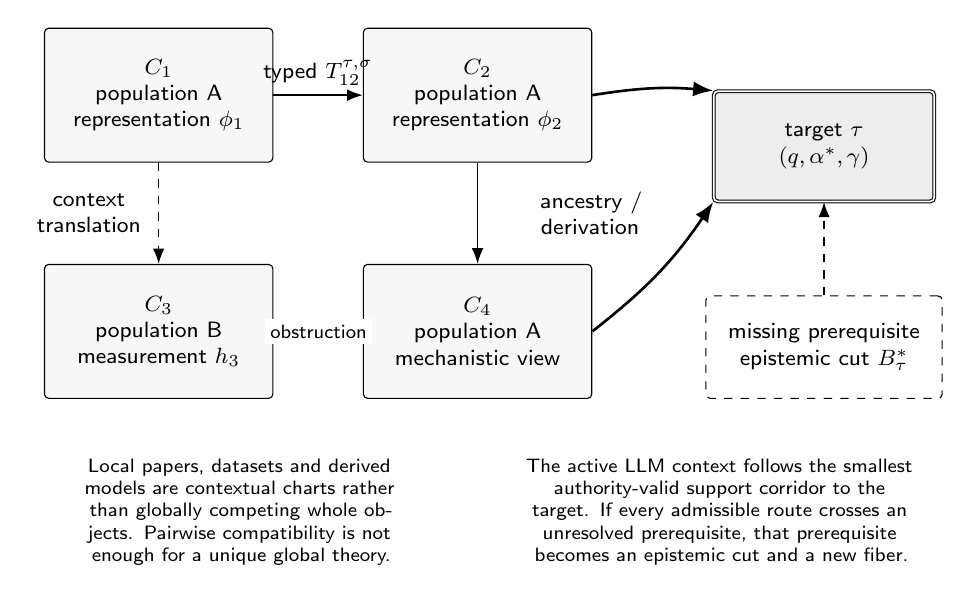
\begin{tikzpicture}[>=Latex,every node/.style={font=\sffamily\footnotesize,align=center},chart/.style={draw,rounded corners=1.5pt,minimum width=29mm,minimum height=17mm,fill=black!3},target/.style={draw,double,rounded corners=1.5pt,minimum width=28mm,minimum height=14mm,fill=black!7},cut/.style={draw,dashed,rounded corners=1.5pt,minimum width=30mm,minimum height=13mm},trans/.style={->,line width=0.6pt},strongpath/.style={->,line width=0.95pt},weak/.style={->,dashed,line width=0.55pt}]
\node[chart] (c1) at (0,1.55) {$C_1$\\population A\\representation $\phi_1$};
\node[chart] (c2) at (4.05,1.55) {$C_2$\\population A\\representation $\phi_2$};
\node[chart] (c3) at (0,-1.45) {$C_3$\\population B\\measurement $h_3$};
\node[chart] (c4) at (4.05,-1.45) {$C_4$\\population A\\mechanistic view};
\node[target] (tau) at (8.45,0.9) {target $\tau$\\$(q,\alpha^*,\gamma)$};
\node[cut] (cut) at (8.45,-1.65) {missing prerequisite\\epistemic cut $B^*_{\tau}$};
\draw[trans] (c1) -- node[above]{typed $T_{12}^{\tau,\sigma}$} (c2);
\draw[weak] (c1) -- node[left,xshift=-1mm]{context\\translation} (c3);
\draw[trans] (c2) -- node[right,xshift=1.5mm,text width=23mm]{ancestry /\\derivation} (c4);
\draw[dashed,line width=0.55pt] (c3.east) -- (c4.west); \node[fill=white,inner sep=2pt,font=\sffamily\scriptsize] at (2.03,-1.45) {obstruction};
\draw[strongpath] (c2.east) to[bend left=7] (tau.north west); \draw[strongpath] (c4.east) to[bend right=9] (tau.south west); \draw[weak] (cut.north) -- (tau.south);
\node[font=\sffamily\scriptsize,text width=45mm,anchor=north west] at (-1.35,-2.95) {Local papers, datasets and derived models are contextual charts rather than globally competing whole objects. Pairwise compatibility is not enough for a unique global theory.};
\node[font=\sffamily\scriptsize,text width=49mm,anchor=north west] at (4.55,-2.95) {The active LLM context follows the smallest authority-valid support corridor to the target. If every admissible route crosses an unresolved prerequisite, that prerequisite becomes an epistemic cut and a new fiber.};
\end{tikzpicture}}
\caption{\textbf{Contextual Knowledge Atlas and target-conditioned inquiry.} Papers, datasets and models become local scientific charts. Typed transitions establish which comparisons and derivations are licensed; unresolved incompatibility remains an obstruction. The active research problem is to find an authority-valid support structure to target $\tau$.}
\label{fig:atlas}
\end{figure}

\subsection{Multi-axis scientific authority}
For claim $c$, scientific authority is represented as
\begin{equation}\alpha(c)=(G_c,R_c,M_c,I_c,D_c),\end{equation}
where the coordinates are scoped certificate sets for grounding/provenance, representation/relation, mechanism ancestry, identification/bounding and decision/QoI usability. Under compatible scope, the induced order is coordinatewise. It is a partial order, not automatically a mathematical lattice: incompatible assumptions, populations or observation operators can obstruct a join.

Cross-axis non-escalation is explicit:
\begin{equation}R\not\Rightarrow M,\qquad D\not\Rightarrow M,\qquad M\not\Rightarrow I.\end{equation}
Thus predictive or observational success does not by itself identify a mechanism; mechanism plausibility does not establish point identification; provenance and citation multiplicity do not create truth or independent evidence.

\subsection{Proposal, verification and update}
The proposal channel
\begin{equation}G_\theta(K_t,a_t)\rightarrow\mathcal P_t\end{equation}
may be implemented by an LLM, symbolic program, human or hybrid. Verification is separate:
\begin{equation}
\begin{aligned}
V(p,e,\gamma)\rightarrow\{&\mathrm{SUPPORTED},\mathrm{REFUTED},\mathrm{PARTIALLY\_IDENTIFIED},\\
&\mathrm{BLOCKED},\CannotCheck\}.
\end{aligned}
\end{equation}
Canonical update is
\begin{equation}K_{t+1}=\mathcal U(K_t,a_t,e_{t+1},V,\mathcal G_t^K).\end{equation}
Negative history is monotone,
\begin{equation}\mathcal H_t^{-}\subseteq\mathcal H_{t+1}^{-},\end{equation}
meaning later evidence can supersede interpretation or scope but cannot erase the historical null/refutation event.

\subsection{Mechanism, measurement and uncertainty}
Mechanistic authority requires an evidence-bearing ancestry such as
\begin{equation}
\begin{aligned}
\text{building blocks}&\to\text{interactions}\to\text{mechanism}\\
&\to\text{mesoscopic state}\to\text{effective law}\to\text{observation/QoI}.
\end{aligned}
\end{equation}
Missing ancestry leads to partial identification or a mechanism set rather than a forced mechanism label.

Measurement is explicit. We write
\begin{equation}y=h(O,\eta,\gamma)+\epsilon,\end{equation}
with $\eta$ representing instrument/calibration state. For affine $Y=AX+b$,
\begin{equation}\mu_Y=A\mu_X+b,\qquad \Sigma_Y=A\Sigma_XA^\top.\end{equation}
For differentiable nonlinear $g$, the first-order approximation
\begin{equation}\Sigma_{g(X)}\approx J_g\Sigma_XJ_g^\top\end{equation}
is explicitly local and assumption-dependent. Root-sum-square uncertainty is accepted only with an independence or uncorrelatedness witness.

\subsection{Recursive fibers, target paths and epistemic cuts}
An unresolved transformation is
\begin{equation}f=(o_f,q_f,\gamma_f,r_f,\operatorname{parent}(f)).\end{equation}
Residual routing opens only dimensions capable of changing the target conclusion. For target $\tau=(q,\alpha^*,\gamma)$, \RAKL{} searches for an authority-valid support subgraph or hypergraph. A conceptual low-cost cut objective is
\begin{equation}B^*_{\tau}=\arg\min_B\operatorname{Cost}(B)\end{equation}
subject to every admissible support route intersecting $B$. This equation defines a research-control target rather than a guarantee that a globally optimal cut always exists or is computationally tractable. A cut may correspond to missing evidence, measurement, context, transition, mechanism, formal lemma or reasoning operator.

\subsection{Action selection, model criticism and assumption sensitivity}
When calibrated probabilities are justified, one admissible policy family is
\begin{equation}u(a\mid K_t)=\frac{\lambda_Q I(Q;Y_a\mid K_t)+\lambda_M\operatorname{Sep}(a,\mathcal V_t)+\lambda_N E[\Delta N_a]}{\operatorname{Cost}(a)}.\end{equation}
Without calibrated probabilities, \RAKL{} uses set-valued alternatives such as worst-case mechanism separation or identified-set shrinkage.

For frozen model criticism, scientific discrepancy probes are $s_k=T_k(y_{\mathrm{obs}})$ and are compared with predictive/generative samples $s_k^{(b)}=T_k(y_{\mathrm{pred}}^{(b)})$. A two-sided finite-sample predictive tail plus a predeclared materiality tolerance can identify a structured residual. Passing the probes establishes adequacy only relative to the frozen probe family, population and resolution; it does not prove truth or mechanism identity.

A complementary assumption-sensitivity operator evaluates a frozen envelope $(a_j,\theta_j)$ under the same context and QoI. For material threshold $\delta$,
\begin{equation}
C(\theta;\delta)=
\begin{cases}
\mathrm{POSITIVE}, & \theta>\delta,\\
\mathrm{NEGATIVE}, & \theta<-\delta,\\
\mathrm{INDETERMINATE}, & |\theta|\le\delta.
\end{cases}
\end{equation}
A baseline conclusion is robust only within the registered envelope when all available preregistered scenarios preserve its material conclusion class. Robustness does not prove the assumptions true; a changed population or QoI is a new contextual chart rather than an assumption perturbation of the same claim.

\section{Bounded scientific cognition}
Canonical archive size and active prompt size are different resources. For operation
\begin{equation}o=(a,f,q,\gamma,\alpha^*,B),\end{equation}
let $M(o)$ denote mandatory epistemic material: target/scope, assumptions, falsifiers, relevant negative history, contradiction sides, authority prerequisites, mechanism ancestry and evaluator/benchmark identity. The compiler defines the constrained objective
\begin{equation}C^*(o)=\arg\max_{C\subseteq V(o)}U(C\mid o),\qquad M(o)\subseteq C,\qquad \operatorname{Tokens}(C)\le B.\end{equation}
The current reference algorithm is a deterministic constrained-coverage heuristic; no global optimality is claimed for arbitrary utilities. If $\operatorname{Tokens}(M(o))>B$, the correct state is \CannotCompile{}, not silent truncation. Compact views remain reconstructable projections with source pointers and erasure metadata.

A key long-project target is archive-scale invariance. For an unchanged scientific target,
\begin{equation}\frac{\partial E[\text{active context tokens}]}{\partial N_{\text{irrelevant archive objects}}}\approx0\end{equation}
while mandatory recall remains one. Frozen known-answer tests add $1\times$, $10\times$ and $100\times$ unrelated distractor records and require identical selected records and active token cost.

\begin{figure}[t]
\centering
\resizebox{0.94\textwidth}{!}{%
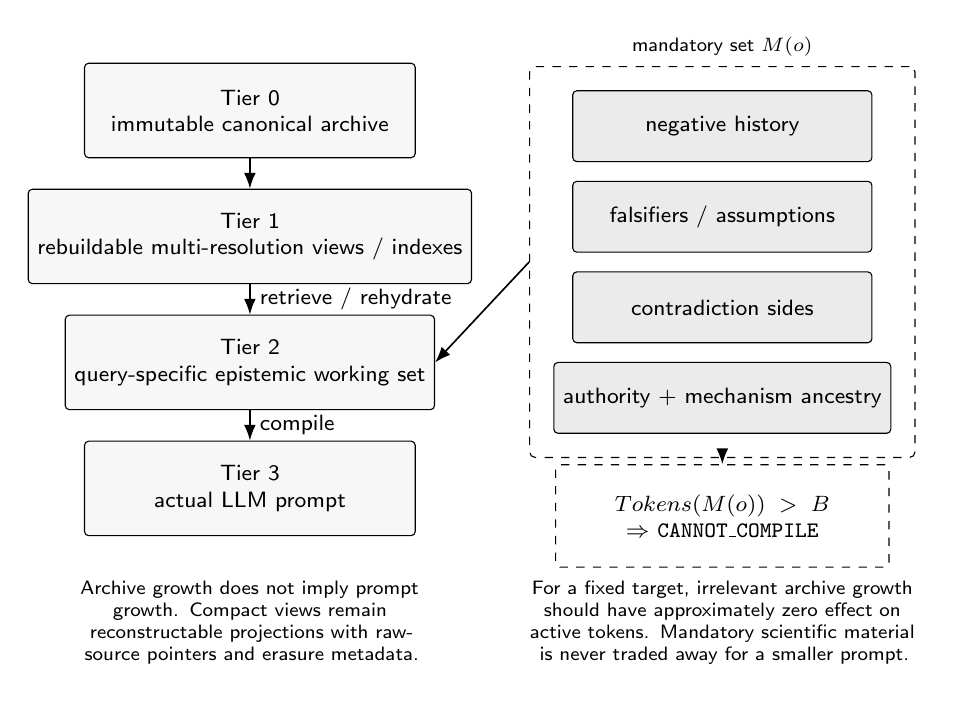
\begin{tikzpicture}[>=Latex,every node/.style={font=\sffamily\footnotesize,align=center},tier/.style={draw,rounded corners=1.5pt,minimum width=42mm,minimum height=12mm,fill=black!3},mandatory/.style={draw,rounded corners=1.5pt,minimum width=38mm,minimum height=9mm,fill=black!8},arrow/.style={->,line width=0.6pt}]
\node[tier] (archive) at (0,2.4) {Tier 0\\immutable canonical archive};
\node[tier] (index) at (0,0.8) {Tier 1\\rebuildable multi-resolution views / indexes};
\node[tier] (working) at (0,-0.8) {Tier 2\\query-specific epistemic working set};
\node[tier] (prompt) at (0,-2.4) {Tier 3\\actual LLM prompt};
\draw[arrow] (archive) -- (index); \draw[arrow] (index) -- node[right]{retrieve / rehydrate} (working); \draw[arrow] (working) -- node[right]{compile} (prompt);
\node[mandatory] (neg) at (6.0,2.2) {negative history}; \node[mandatory] (fals) at (6.0,1.05) {falsifiers / assumptions}; \node[mandatory] (contr) at (6.0,-0.10) {contradiction sides}; \node[mandatory] (anc) at (6.0,-1.25) {authority + mechanism ancestry};
\node[draw,dashed,rounded corners=2pt,fit=(neg)(anc),inner sep=3mm,label={[font=\sffamily\scriptsize]above:mandatory set $M(o)$}] (mand) {};
\draw[arrow] (mand.west) -- (working.east);
\node[draw,dashed,rounded corners=1.5pt,text width=40mm,minimum height=13mm] (fail) at (6.0,-2.75) {$Tokens(M(o))>B$\\$\Rightarrow$ \texttt{CANNOT\_COMPILE}};
\draw[arrow,dashed] (mand.south) -- (fail.north);
\node[font=\sffamily\scriptsize,text width=45mm,anchor=north] at (0,-3.45) {Archive growth does not imply prompt growth. Compact views remain reconstructable projections with raw-source pointers and erasure metadata.};
\node[font=\sffamily\scriptsize,text width=50mm,anchor=north] at (6.0,-3.45) {For a fixed target, irrelevant archive growth should have approximately zero effect on active tokens. Mandatory scientific material is never traded away for a smaller prompt.};
\end{tikzpicture}}
\caption{\textbf{Bounded scientific cognition.} The archive and method history can grow while the model sees only a target-specific working set. Some atoms are mandatory because dropping them changes epistemic validity. If they cannot fit, the operation fails closed rather than silently compressing them away.}
\label{fig:context}
\end{figure}

\section{Learning and evolving the method}
\subsection{Challenge Learning}
Metacognitive diagnosis is separated from learning control, consistent with recent calls to treat monitoring, evaluation, control and adaptation as distinct AI self-governance functions \cite{ji2026}. A failure is attributed to a candidate cause such as missing evidence, implementation defect, stochastic or underpowered result, wrong strategy, ontology/context gap or method-basis gap. The controller can recommend persistence, strategy switching, help seeking, evidence acquisition, implementation repair, a discriminating challenge, or operator invention/assimilation. A simple learning-progress signal is
\begin{equation}LP_t(f)=Q_t(f)-Q_{t-k}(f).\end{equation}
Failure attribution is important: a missing measurement is not automatically a missing reasoning operator.

\subsection{Assimilation and constructive invention}
An external method is decomposed into an atomic contract
\begin{equation}C_m=(I_m,O_m,\gamma_m,A_m,P_m,F_m,\alpha_m^+,\alpha_m^-,T_m,B_m),\end{equation}
recording inputs, outputs, context, assumptions, preconditions, failures, authority it may and may not create, transitions and benchmark identity. A candidate may be equivalent to an incumbent, a parallel local view, shadow-eligible, blocked or rejected. External reputation is not imported as authority. Constructive invention is likewise proposal-only; a new formalism must state variables, interactions, observation map, limiting cases, assumptions, predictions and falsifiers before target evidence can support it.

\subsection{Governed Self-RAKL}
For incumbent method $M_t$ and challenger $M'$, development improvement
\begin{equation}\Delta_D=q_D(M')-q_D(M_t)>0\end{equation}
is local optimization only. Strong scoped evolution evidence additionally requires fresh assurance
\begin{equation}\Delta_A=q_A(M')-q_A(M_t)>0,\end{equation}
with frozen candidate/evaluator chronology, matched resources, preserved negative history and all blocking invariants clean. Repeated exposure to the assurance set consumes its evidential value, a concern related to adaptive holdout reuse \cite{dwork2015}. Development improvement with assurance regression is \texttt{META\_OVERFIT}.

\begin{figure}[t]
\centering
\resizebox{\textwidth}{!}{%
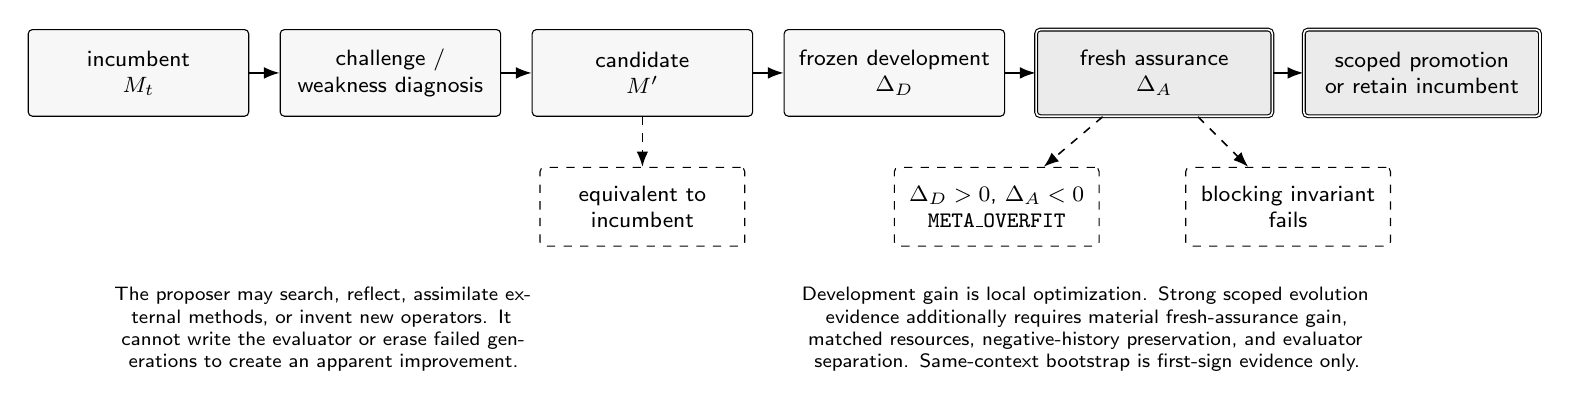
\begin{tikzpicture}[>=Latex,every node/.style={font=\sffamily\footnotesize,align=center},stagebox/.style={draw,rounded corners=1.5pt,minimum width=28mm,minimum height=11mm,fill=black!3},guard/.style={draw,double,rounded corners=1.5pt,minimum width=30mm,minimum height=11mm,fill=black!8},bad/.style={draw,dashed,rounded corners=1.5pt,minimum width=26mm,minimum height=10mm},arrow/.style={->,line width=0.6pt},dashedarrow/.style={->,dashed,line width=0.55pt}]
\node[stagebox] (m0) at (0,0) {incumbent\\$M_t$}; \node[stagebox] (challenge) at (3.2,0) {challenge /\\weakness diagnosis}; \node[stagebox] (candidate) at (6.4,0) {candidate\\$M'$}; \node[stagebox] (dev) at (9.6,0) {frozen development\\$\Delta_D$}; \node[guard] (assure) at (12.9,0) {fresh assurance\\$\Delta_A$}; \node[guard] (promote) at (16.3,0) {scoped promotion\\or retain incumbent};
\draw[arrow] (m0) -- (challenge); \draw[arrow] (challenge) -- (candidate); \draw[arrow] (candidate) -- (dev); \draw[arrow] (dev) -- (assure); \draw[arrow] (assure) -- (promote);
\node[bad] (equiv) at (6.4,-1.7) {equivalent to\\incumbent}; \node[bad] (overfit) at (10.9,-1.7) {$\Delta_D>0$, $\Delta_A<0$\\\texttt{META\_OVERFIT}}; \node[bad] (blocked) at (14.6,-1.7) {blocking invariant\\fails};
\draw[dashedarrow] (candidate) -- (equiv); \draw[dashedarrow] (assure) -- (overfit); \draw[dashedarrow] (assure) -- (blocked);
\node[font=\sffamily\scriptsize,text width=60mm,anchor=north west] at (-0.8,-2.6) {The proposer may search, reflect, assimilate external methods, or invent new operators. It cannot write the evaluator or erase failed generations to create an apparent improvement.};
\node[font=\sffamily\scriptsize,text width=72mm,anchor=north west] at (8.3,-2.6) {Development gain is local optimization. Strong scoped evolution evidence additionally requires material fresh-assurance gain, matched resources, negative-history preservation, and evaluator separation. Same-context bootstrap is first-sign evidence only.};
\end{tikzpicture}}
\caption{\textbf{Governed self-evolution.} A candidate can be generated endogenously or assimilated from external work, but development gain is insufficient. Strong scoped evolution evidence requires fresh assurance outside the challenger's write authority. Failed, equivalent, blocked and overfit generations remain in the lineage.}
\label{fig:selfevolution}
\end{figure}

\section{Reference implementation and scoped formal closure}
The current reference profile registers exactly 24 high-impact method surfaces: decomposition; routing; search/query generation; source selection/reliability; claim extraction; ontology/terminology normalization; mathematical/context translation; equivalence/similarity; contextual theory gluing; contradiction diagnosis; gap discovery; experiment/query selection; synthesis; memory; review; benchmarking; authority promotion; saturation/stopping; prompting/context policy; capability shaping; software architecture/execution; research portfolio/tree control; objective evolution; and generator transport.

For each surface $m$, a machine-readable contract $C(m)$ contains typed inputs/outputs, context, assumptions, state read/write sets, authority effect, non-escalation rules, failure semantics, invariants, mathematical semantics, implementation/test references and explicit empirical-open coordinates. We define scoped formal closure for reference profile $\mathcal R$ as
\begin{equation}\operatorname{FormalClosed}_{\mathcal R}(M)=\mathbf 1\!\left[\forall m\in\mathcal M,\;\exists!C(m):\operatorname{ContractValid}(C(m))\right].\end{equation}
This is a structural property only. It does not establish empirical superiority, global method completeness or scientific saturation. New child operators must declare ownership under existing surfaces or reopen the high-level inventory.

The implementation includes content-addressed project storage, bounded task packets, exact execution specifications, immutable receipts, release manifests, token-count certificates, measurement-aware relation checks, a canonical historical meta-fiber compiler, method assimilation, constructive invention, challenge learning, model criticism, assumption sensitivity and coding-agent adapters. Runtime attestation binds observed executable bytes and declared-environment fingerprints as reproducibility evidence, not scientific truth.

At exact implementation-stage candidate \ImplementationSHA{}, the GitHub Actions workflow completed with \SoftwareTests{} passing tests. These tests establish software-contract behavior on frozen known-answer and hostile worlds; they are not evidence of real-world scientific superiority.

\paragraph{Current evidence boundary.} The formal/mechanic inventory and software known-answer contracts are executed. Archive-scale context invariance is currently synthetic/known-answer evidence. Same-context self-correction is observed but receives no independent-review credit. Matched-workflow superiority, fresh-assurance self-evolution, independent replication and the real spot/Polymarket scientific result remain unexecuted or preregistered. This preprint therefore reports a method and its current software evidence, not a completed empirical superiority claim.

\section{First-sign Self-RAKL evidence}
Applying the method to itself has already exposed several real defects: same-context expert roles had initially been too easy to confuse with independent review; storage and prompt growth had not been sufficiently separated; metacognitive diagnosis did not yet determine how the system should learn; missing method operators had not been clearly separated from missing evidence or implementation defects; historical meta-fiber identifiers collided; and recent cross-domain model-discovery review exposed implicit model-criticism and assumption-sensitivity mechanics that needed explicit executable contracts. The canonical historical-ledger compiler also rejected incorrect Round-42 fiber allocations during this preprint preparation.

These are useful first-sign self-correction results because the framework's own controls caught and repaired problems in its representation and method. They are not strong self-evolution evidence: the work shares one overall orchestration context and has not yet executed the frozen fresh-assurance coding-agent bootstrap benchmark. When the current same-context evidence is evaluated against the strong bootstrap contract, missing registered development/fresh-assurance quantities correctly prevent the strong verdict rather than being silently inferred.

\section{Preregistered empirical evaluation}
\subsection{Matched scientific-research workflows}
The same base LLM will be compared under matched evidence cutoff, tools, hidden outcomes and resource budget across direct strong prompting, retrieval-augmented research, a strong generic agentic workflow, fixed \RAKL{} and self-evolving \RAKL{}. Primary outcomes include hidden scientific-defect precision/recall, unsupported authority upgrades, counterevidence uptake, negative-history recovery, experiment discrimination per cost, final held-out scientific performance, context tokens, tool calls and wall time. The framework loses its empirical case if simpler conditions match its registered scientific-process and final-task outcomes at lower cost without more blocking failures.

\subsection{Fresh-assurance self-evolution}
Sealed method-defect worlds are reconstructed from real research failures while withholding the defect label. Candidate classes include target leakage, misspecified correspondence nulls, missing replication, multiplicity, estimand mismatch and causal-clock overreach. A strong self-evolution result requires localization of a previously unlabelled weakness, a discriminator frozen before repair, a non-equivalent candidate and material transfer on fresh assurance. Development-only gains are insufficient.

\subsection{Real quant-finance study}
The real application is the existing \texttt{polymarket\_crypto} research programme. The scientific order is deliberately spot-first:
\begin{equation}
\begin{aligned}
\text{spot evidence}&\to\text{descriptive spot atlas}\to\text{predictive 5/15-minute spot path}\\
&\to\text{oracle/contract transform}\to\text{downstream Polymarket}.
\end{aligned}
\end{equation}
Polymarket features are excluded from the primary spot model and cannot repair a failed spot-science result.

The descriptive target covers return/displacement distributions, volatility and volatility-of-volatility, tails/jumps, activity/duration, continuation/reversal/memory, local microstructure/liquidity, global crypto state, cross-asset/venue dependence and observation/clock state. Model criticism will use frozen discrepancy probes so that ``fully explain'' means no registered scientifically material structured residual remains at the declared scope, not deterministic reproduction of every market tick. Assumption sensitivity will separately evaluate fragility to preregistered clock, missingness, nuisance, dependence and transport scenarios.

The predictive object is a future spot-path distribution at 5 and 15 minutes. On identical causal rows, a central bridge estimand is
\begin{equation}\Delta_{\mathrm{joint}}=\min(R_D,R_G)-R_{DG},\end{equation}
where $R_D$, $R_G$ and $R_{DG}$ are strictly proper predictive risks for microstructure-only, global-only and joint states. A positive joint result requires a preregistered material threshold, multiplicity-aware positive lower confidence bound on untouched or forward evidence, calibration and transport checks. A simpler lawful parent winning is a valid scientific result.

Exploration may deliberately fit high-capacity overfit teacher models as structure detectors. Teacher fit has proposal authority only. \RAKL{} probes what the teacher exploits, removes leakage/nuisance features, extracts stable interactions, formulates mathematical successors and confirms only frozen descendants on untouched evidence.

\section{Discussion and falsifiers}
\RAKL{} is intended as a scientific authority and research-control layer around a replaceable LLM, not a claim that one agent architecture has solved scientific reasoning. The architecture externalizes evidence-bearing knowledge, explanatory models, procedural skills, a research agenda, failure history, metacognitive control and resource constraints. Human-inspired terms are operationalized rather than anthropomorphized: intellectual humility becomes evidence-triggered revision, curiosity becomes information gain or learning-progress exploration, reflection becomes diagnosis plus a costed control action, and experience becomes a reusable skill only after transfer.

The self-bootstrap requirement is not circular because self-application is separated from self-authorization. \RAKL{} may discover a weakness in itself and propose a repair, but acceptance comes from a frozen harness and fresh tasks outside the challenger's control. Formal closure likewise does not mean the method is finished forever. It means the current registered high-impact inventory has no known unowned specification surface. The Polymarket/spot project is deliberately the next integration stress test. If that project exposes a high-impact operation absent from the current 24-surface system, the correct outcome is to reopen scoped formal closure.

The paper registers direct falsifiers. If direct prompting, RAG or a simpler agent workflow matches \RAKL{} on registered process and final-task outcomes at lower cost without more validity failures, the framework complexity is not justified. If removing a mechanism does not selectively worsen its preregistered failure mode, that mechanism's contribution is unsupported. If method changes improve only development tasks, the strong self-evolution claim fails. If a simpler context policy matches mandatory evidence retention and task quality under matched budgets, the complex compiler has not earned its cost. If the registered quant information set contains no material 5/15-minute predictive information after causal controls, \RAKL{} must report that ceiling or the missing observable rather than search until significance appears. If semantically equivalent prior work is found, the novelty claim narrows regardless of terminology.

\section*{Reproducibility and AI-use statement}
The public repository is \url{https://github.com/SzeChunYiu/RAKL}. It maintains frozen benchmarks, content-addressed execution receipts, exact-subject CI, negative-history records, release manifests and editable paper/figure sources. Language models are research, coding and drafting tools rather than authors; their proposals do not possess canonical scientific authority. Same-context role simulations are not counted as independent peer review. The later journal-results manuscript will bind exact data/transformation identities, model-run receipts and all quantitative figure source data.

\appendix
\section{Structural proof obligations}
Core proof/test obligations include generation non-authority, mechanism non-upgrade, typed relation non-escalation, non-forced gluing, negative-history monotonicity, conservative evidence-lineage saturation, missing-evidence honesty, residual reopening, meta-evaluator separation, measurement non-escalation, explicit uncertainty assumptions and formal-closure honesty. These are structural constraints on the method; they do not prove empirical scientific performance.

\begin{thebibliography}{99}
\bibitem{alzubi2026} S. Alzubi, N. Provenzano, J. Bingham, W. Chen, and T. Vu. EvoSkill: Automated Skill Discovery for Multi-Agent Systems. arXiv:2603.02766, 2026.
\bibitem{dogah2026} W. Dogah. Traxia: A Framework for Verifiable, Agent-Native Scientific Publishing. arXiv:2606.08256, 2026.
\bibitem{dwork2015} C. Dwork, V. Feldman, M. Hardt, T. Pitassi, O. Reingold, and A. Roth. The reusable holdout: Preserving validity in adaptive data analysis. \emph{Science}, 349(6248):636--638, 2015. doi:10.1126/science.aaa9375.
\bibitem{gao2026} X. Gao, C. Hu, H. Chen, et al. EvoAgentBench: Benchmarking Agent Self-Evolution via Ability Transfer. arXiv:2607.05202, 2026.
\bibitem{ghafarollahi2024} A. Ghafarollahi and M. J. Buehler. SciAgents: Automating scientific discovery through multi-agent intelligent graph reasoning. arXiv:2409.05556, 2024.
\bibitem{ghareeb2026} A. E. Ghareeb, B. Chang, L. Mitchener, et al. A multi-agent system for automating scientific discovery. \emph{Nature}, 655:497--505, 2026. doi:10.1038/s41586-026-10652-y.
\bibitem{gibson2026} J. Gibson. Sheaves as a Means of Maintaining Consistency in Model-based Systems Engineering. arXiv:2605.08609, 2026.
\bibitem{gottweis2026} J. Gottweis, W.-H. Weng, A. Daryin, et al. Accelerating scientific discovery with Co-Scientist. \emph{Nature}, 655:487--496, 2026. doi:10.1038/s41586-026-10644-y.
\bibitem{ji2026} E. Y. Ji, I. Grossmann, and A.-H. Karimi. Metacognition Should Be the Scientific Framework for Bounded and Effective Self-Governance in Generative AI. arXiv:2605.23981, 2026.
\bibitem{jiang2023} H. Jiang, Q. Wu, C.-Y. Lin, Y. Yang, and L. Qiu. LLMLingua: Compressing Prompts for Accelerated Inference of Large Language Models. In \emph{EMNLP}, pages 13358--13376, 2023. doi:10.18653/v1/2023.emnlp-main.825.
\bibitem{mitchener2025} L. Mitchener, A. Yiu, B. Chang, et al. Kosmos: An AI Scientist for Autonomous Discovery. arXiv:2511.02824, 2025.
\bibitem{packer2023} C. Packer, S. Wooders, K. Lin, V. Fang, S. G. Patil, I. Stoica, and J. E. Gonzalez. MemGPT: Towards LLMs as Operating Systems. arXiv:2310.08560, 2023.
\bibitem{riosgarcia2026} M. Rios-Garcia, N. Alampara, C. Gupta, I. Mandal, S. Mannan, A. A. Aghajani, N. M. A. Krishnan, and K. M. Jablonka. AI scientists produce results without reasoning scientifically. arXiv:2604.18805, 2026.
\bibitem{sarthi2024} P. Sarthi, S. Abdullah, A. Tuli, S. Khanna, A. Goldie, and C. D. Manning. RAPTOR: Recursive Abstractive Processing for Tree-Organized Retrieval. \emph{ICLR}, 2024.
\bibitem{shen2026} S. Shen, W. Cheng, M. Ma, A. Turcan, M. J. Zhang, and J. Ma. SkillFoundry: Building Self-Evolving Agent Skill Libraries from Heterogeneous Scientific Resources. arXiv:2604.03964, 2026.
\bibitem{skarlinski2024} M. D. Skarlinski, S. Cox, J. M. Laurent, J. D. Braza, M. Hinks, M. J. Hammerling, M. Ponnapati, S. G. Rodriques, and A. D. White. Language agents achieve superhuman synthesis of scientific knowledge. arXiv:2409.13740, 2024.
\bibitem{souza2025} R. Souza, A. Gueroudji, S. DeWitt, D. Rosendo, T. Ghosal, R. Ross, P. Balaprakash, and R. Ferreira da Silva. PROV-AGENT: Unified Provenance for Tracking AI Agent Interactions in Agentic Workflows. arXiv:2508.02866, 2025.
\bibitem{vitali2026} F. Vitali and V. Pasqual. Provenance-Enhanced Statements in Knowledge Graphs. arXiv:2606.15246, 2026.
\bibitem{xu2023} F. Xu, W. Shi, and E. Choi. RECOMP: Improving Retrieval-Augmented LMs with Compression and Selective Augmentation. arXiv:2310.04408, 2023.
\bibitem{yamada2025} Y. Yamada, R. T. Lange, C. Lu, S. Hu, C. Lu, J. Foerster, J. Clune, and D. Ha. The AI Scientist-v2: Workshop-Level Automated Scientific Discovery via Agentic Tree Search. arXiv:2504.08066, 2025.
\bibitem{zhang2025} J. Zhang, S. Hu, C. Lu, R. Lange, and J. Clune. Darwin Godel Machine: Open-Ended Evolution of Self-Improving Agents. arXiv:2505.22954, 2025.
\end{thebibliography}

\end{document}
